% #############################################################################
% This is Chapter 8
% !TEX root = ../main.tex
% #############################################################################
% Change the Name of the Chapter i the following line
\fancychapter{Conclusion}
% The following line allows to ref this chapter
\label{chap:conclusion}

This chapter concludes the dissertation by reflecting on the development and application of the proposed method for deriving stakeholder-specific architecture viewpoints and generating their corresponding views. It summarises the main outcomes of the \ac{DORA} demonstrations and discusses the considerations arising from the use of \ac{GenAI}, operational evidence, and stakeholder feedback. The chapter then outlines opportunities for further development, addressing refinements to the methodology and its artefacts, extensions to the regulatory scope, and the maintenance of architectural representations as legal requirements evolve.

% #############################################################################
\section{Outcomes and Considerations}

Overall, the method presented positive outcomes in a myriad of ways. The extraction of concerns and operational footprint were faithful to the realities of the interviewed stakeholders. The selection of relevant articles and corresponding breakdown of requirements, all the while maintaining traceability "in check" also achieved satisfactory levels.

Defined viewpoints formed a basis for view generation. The positive reception of generated views by the stakeholders is preliminary evidence of viewpoint relevance and comprehensibility. If viewpoints did not correctly define the rules for formulating stakeholder relevant views, the views themselves would not have received positive feedback.

The use of \ac{GenAI} throughout the methodology highlights the importance of maintaining human judgement within the modelling process. Automated assistance supports the extraction, organisation, and representation of information, while the user reviews the proposed interpretations and approves their inclusion. Traceability and cross-artifact reconciliation support this responsibility by making the origins of represented information and the consistency of its use inspectable.

A further consideration is the dependence of stakeholder-specific viewpoints on the information made explicit during elicitation. An activity or control omitted from an interview may remain unrepresented or have unclear ownership, even when it exists in practice. The demonstration illustrated how presenting a view back to its stakeholder can reveal such omissions and prompt clarification. Generated views therefore serve both as representations of the available evidence and as instruments for enriching that evidence through discussion. The preliminary feedback supports this iterative role, while broader assessment involving additional stakeholders and independent reviewers would help establish how consistently the methodology supports understanding across different organisational and regulatory contexts.

Regardless, further improvements and refinements can be made on the current state of the methodology, as well as extending the current scope of produced artifacts. Feedback gathered from real, external stakeholders provided valuable insights regarding what produced artifacts hold the most value. The future work section (\ref{FWork}) provides further insights on what could be improved on the model.

% #############################################################################
\section{Future Work}
\label{FWork}

\subsection{Improvements on the method}

In its current state, the methodology can generate structurally valid ArchiMate views, including meaningful requirement groupings and semantic containment. However, the visual layout of the generated views remains only partially automated. Although elements are positioned so that they do not overlap, their placement is not yet optimised to communicate the underlying structure clearly or to support efficient interpretation by stakeholders.

As a result, relationships may cross unrelated elements or other relationships, and long connectors may reduce the readability of the view. The generated models also do not yet make systematic use of connector bend points or routing strategies to improve the visual separation of relationships. Consequently, a manual layout clean-up step is still required before the views can be considered presentation-ready.

Future work could improve either the direct model-generation mechanism or introduce a dedicated post-processing layout stage. Such work could apply layout rules based on element type, containment, relationship direction, and stakeholder reading paths, while automatically routing connectors to minimise crossings. This would reduce the manual effort required after generation, improve the readability of the resulting views, and make the methodology faster to apply in practice.

As per the received feedback indicates, the generated textual explanations of views require additional work to deliver the full scope of the potential value they hold, namely changing the current scope of explanation from the methodology to the operational footprint of the designated stakeholder.

Regarding the regulations used, this work deliberately left out regulatory and implementing technical standards, which limits the output produced by the methodology. Detailed requirements concerning, for example, \ac{ICT} change management, testing environments, source-code testing, and logging are represented only where they follow directly from the text of \ac{DORA} itself, and not from the supplementary technical standards. Thus, incorporation of \ac{RTS} and \ac{ITS} constitutes a possible extension of the methodology.

Additionally, it is worth noting that this work is in ArchiMate 3.2. Archimate 4 has been released on April of 2026, so future work must also update the agents and skills of the pipeline to produce artifacts oriented towards ArchiMate 4.

\subsection{Traceability Matrix}

The traceability matrix can still be further refined. Automation parsing currently exhibits limitations regarding amendments, and the current state of the software outputs erroneous \ac{ID}s when evaluating them, due to being structured very differently from the rest of the document. This upgrade would facilitate the automated generation of a traceability matrix of  a document that is mostly made-up of amendments, such as \ac{eIDAS2}. Due to this, the current \ac{ID} system would also need to be revisited, since in the current state it is incapable of housing enough identifiers to uniquely identify text of documents with amendments, taking into account that these introduces additional hierarchical tiers. An example of this can be seen in \ac{eIDAS2}, where an original provision is immediately succeeded by its amendatory text, within the original article, something that is not representable with the current \ac{ID} system. An example can be seen in figure \ref{fig:amendEx}.

\begin{figure}[H]
  \centering
  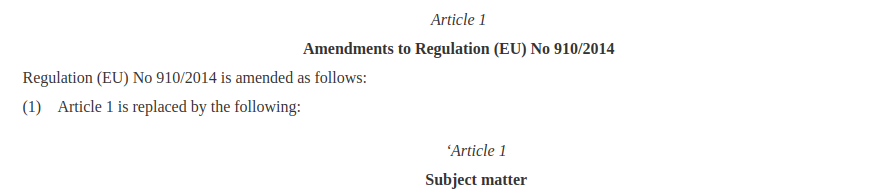
\includegraphics[width=1\textwidth]{Images/AmendmentExampleeIDAS2.png}
  \caption{Example of an excerpt from \ac{eIDAS2} that is indescribable with the current \ac{ID} system}
  \label{fig:amendEx}
\end{figure}

\subsection{Enterprise Gap Detection}

While the focus of the current method is the identification and formalization of viewpoints of a stakeholder regarding an \ac{EU} act, and then materializing said viewpoints into views with the purpose of informing the stakeholder about how the legislation impacts their operational footprint, the method can be taken further extended. While an interview of a single enterprise employee is not sufficient evidence to state if the company has a gap in relation to the legislation (due to the stakeholder either not being in scope of a given requirement, or simply not being informed of it), the potential to do so indicates considerable potential. In fact, a hypothesis may be that if a multitude of viewpoints from different employees indicates a gap, the gap probably exists in the enterprise. The method could be evolved into conducting interviews with multiple employees of the same role, and crossing the results in order to identify gaps within a company in regards to a certain legislation. 

\subsection{Version Aware Regulatory Maintenance}

The methodology currently preserves a traceability matrix for the selected consolidated regulation. Future work could extend this capability into a version-aware maintenance mechanism. The mechanism could record the source version and effective date of the regulation, compare later consolidated versions, and identify which legal requirements, coverage records, viewpoints, and models are affected by a legal change. Rather than repeating the complete pipeline after every amendment, only the artifacts connected to changed legal provisions would require review. This would improve the long-term applicability of the methodology for regulations that evolve frequently.